\documentclass[12pt, letterpaper]{article}
\usepackage[titletoc,title]{appendix}
\usepackage{color}
\usepackage{booktabs}
\usepackage{caption}
\newcommand\fnote[1]{\captionsetup{font=small}\caption*{#1}}

\usepackage[usenames,dvipsnames,svgnames,table]{xcolor}
\definecolor{dark-red}{rgb}{0.75,0.10,0.10} 
\usepackage[margin=1in]{geometry}
\usepackage[linkcolor=dark-red,
			colorlinks=true,
			urlcolor=blue,
			pdfstartview={XYZ null null 1.00},
			pdfpagemode=UseNone,
			citecolor={dark-red},
			pdftitle={Consumption of Pornography Online}]{hyperref}
\usepackage{multibib}
\usepackage{geometry} % see geometry.pdf on how to lay out the page. There's lots.
\geometry{letterpaper}               % This is 8.5x11 paper. Options are a4paper or a5paper or other... 
\usepackage{graphicx}                % Handles inclusion of major graphics formats and allows use of 
\usepackage{amsfonts,amssymb,amsbsy}
\usepackage{amsxtra}
\usepackage{natbib}
\usepackage{dcolumn}
\usepackage{longtable}
\usepackage{verbatim}
\setcitestyle{round,semicolon,aysep={},yysep={;}}
\usepackage{setspace}		     % Permits line spacing control. Options are \doublespacing, \onehalfspace
\usepackage{sectsty}		     % Permits control of section header styles
\usepackage{lscape}
\usepackage{fancyhdr}		     % Permits header customization. See header section below.
\usepackage{url}                 % Correctly formats URLs with the \url{} tag
\usepackage{fullpage}		     %1-inch margins
\usepackage{multirow}
\usepackage{rotating}
\setlength{\parindent}{3em}
\usepackage{subcaption}
\usepackage[T1]{fontenc}
\usepackage{bm}
\usepackage{libertine}

\usepackage{chngcntr}


\title{\Large{Consumption of Pornography Online}\footnote{Data and scripts behind the analysis presented here can be downloaded at: \href{http://github.com/soodoku/porn}{http://github.com/soodoku/porn.}}}

\author{Gaurav Sood\thanks{Gaurav can be reached at \href{mailto:gsood07@gmail.com}{\footnotesize{\texttt{gsood07@gmail.com}}}} \and Andrew Guess\thanks{New York University, \href{mailto:guess@nyu.edu}{\footnotesize{\texttt{guess@nyu.edu}}}}\vspace{.5cm}}

\date{\vspace{.5cm}\normalsize{\today}}

\begin{document}
\maketitle

\begin{center}
\vspace{.5cm}\textbf{NB:} Preliminary draft. Please do not cite without permission.\vspace{1.5cm}
\end{center}

\begin{comment}

setwd(paste0(basedir, "adult/ms"))
tools::texi2dvi("porn.tex", pdf=TRUE, clean=TRUE) 
setwd(basedir)

\end{comment}

\begin{abstract}
\noindent Consumption of pornography has been blamed for a variety of societal ills, including, rise in misogyny, sex crimes, and coarsening of the culture. In this paper, using passive browsing data from comScore and YouGov, we investigate how much pornography Americans consume online, how consumption of pornography online has changed over time, and shed light on who consumes pornography. We find that there is a sharp positive skew in the consumption of pornography, with a small number of users consuming lots of pornography and many consuming small amounts. The median Internet user today spends X\% of time consuming pornography, and visits Y sites per year. Between 2002 and 2014, the consumption of pornography online increased by between XX and YY\%. Lastly, we find that, unlike previous data, relying on ecological inference, liberals consume more pornography than conservatives \citep{macinnis2015american, edelman2009markets}.
\end{abstract} 
\clearpage
\doublespace

Consumption of pornography is associated with a variety of disturbing attitudes, beliefs, emotions, and behaviors. Consuming pornography is associated with support for violence against women \citep{hald2010pornography, malamuth2012pornography, donnerstein1984pornography}, belief in rape myths \citep{foubert2011pornography}, greater gender role conflict and lesser sexual satisfaction \citep{szymanski2014psychological, stewart2012young}, poorer relationship quality \citep{szymanski2014psychological, szymanski2015male}, and sexually risky behaviors such as engaging in paid sex, and having extramarital sex \citep{wright2012internet}. A lot of popular pornography also contains a healthy dose of violence. One analysis of popular pornography revealed that 88.2\% of the analyzed scenes contained physical aggression, and 48.7\% verbal aggression \citep{bridges2010aggression}. In all, there exist good reasons to be worried about rise in consumption of pornography.

In this paper, using passive browsing data from comScore and a YouGov sample, we investigate how much pornography do Americans consume online, how consumption of pornography online has changed over time, and shed light on who consumes pornography. We find that there is sharp skew in the consumption of pornography, with a small set of users consuming a large chunk of pornography. The median Internet user today spends X\% of time consuming pornography, and visits Y sites per year. Between 2002 and 2014, the consumption of pornography online has increased by between XX and YY\%. Lastly, we find that, unlike previous data, relying on ecological inference, liberals consume more pornography than conservatives \citep{macinnis2015american, edelman2009markets}. 

\citep{lykke2015widening}
\citep{boik2016empirical}

\section*{Data}
We exploit data from comScore and a YouGov survey to measure the consumption of adult content. 

comScore maintains a panel of around 100,000 households, offering small rewards in exchange for monitoring all Internet data from a machine. There are multiple notable biases in the sample. See \ref{si1_comscore} for comparison between demographics and population benchmarks on some key variables.

YouGov maintains a large online panel recruited through a variety of methods. It uses matched sampling to survey respondents: The provider first draws a random sample from a large synthetic representative sampling frame, finds respondents that match the sampled individuals from its panel, and invites them to take a survey. For details and validation, see \citet{rivers2009}. For this particular sample, panelists also provided de-identified access to their web browsing activity via passive metering software installed voluntarily on their computers. The software, called Wakoopa, can be uninstalled at any point and captures visited web URLs independent of the type of browser or browser-specific privacy settings.\footnote{Wakoopa does not save passwords or financial transactions, and personally identifying information is screened out by the survey provider.} At the time this data was made available in March 2015, YouGov had recruited 1,392 individuals to the web tracking panel, which is currently marketed as YouGov Pulse. Our data comes from \citet{guess2016}. See \ref{si2_yougov} for a comparison between demographics and population benchmarks on some key variables.

The passive metering component of this particular opt-in panel adds a layer of selectivity to the sampling process. Thus, to address concerns about the non-probability sampling procedure, we use raking weights to account for under- or overrepresentation along the following dimensions: age, gender, race, party identification, and region. We obtain population benchmark estimates from the U.S. Census (resident population, 2014) and proportions of party identifiers from Pew (2014). Raking takes into account the marginal, not the joint, distribution of the relevant demographic variables used to estimate the weights.

\section*{Measuring Consumption of Adult Content}
For both comScore and YouGov, we only observe data from a single machine per person. Our analyses should hold if people exhibit similar consumption patterns across devices. If that is too implausible an assumption, then we must decide on the direction of error and how it affects our analyses. We think it is likely that people would be less likely to search for pornography from machines on which they have installed these passive monitoring software (though the data are de-identified). If that is so, our estimates are a lower bound of net consumption of pornography per machine. As number of devices per person are increasing, all these numbers need to be adjusted. Next, is measurement error correlated with ideology? We have little reason to expect that, but we have no capacity to check if it is true. Thus, for current purposes, we assume that it is so. 

We code pornographic content at the domain level. For both YouGov and comScore, we measure ideology using shallalist, DMOZ, and two machine learning classifiers. For YouGov data, we also present data based on classification from Wakoopa. 

Our first classifier is based on just the domain name and domain suffix. In particular, we use a calibrated keyword classifier. The features of the model are whether any of the following keywords are present in the domain name:

\begin{quote}
cumshot, dildo, anal, adult, porn, mature, sex, xx, bbw, slut, whore, tits, titty, titties, pussy, sperm, gay, cheat, booty, ebony, asian, brazilian, fuck, cock, cunt, lesbian, shemale, boob, naughty, fatty, bitch, granny, jizz, faggot, horny, bukakke, bdsm, vagina, smut, x-rated, lusty, erotic, cunnilingus, blowjob, panty, hentai, latex, fetisch, fetish, erotik, bondage, naked, strip, teen, stocking, coitus, deprav, tube, perverse 
\end{quote}

For the 2004 comScore data, this gave about 140k domains that potentially carry pornographic content. We compare this list to the approximately 850k porn domains in the shallalist. This leaves us with a list of 68k domains with uncertain status. Use one of the many URL classification APIs. Using Trusted Source API, we get about 20k porn, and 48k non-porn. This gives us the lower bound of adult domains. 

To estimate the false positives, we take a large random sample of 10,000 unique domains and compare results from our classifier to results from a commercial API by McAfee. This serves are our estimate of the false positive rate. For comScore data, our false negative rate is 5\%. False positive rate is close to 0. All of this ignores pornography available via more conventional channels. For instance, a large amount of pornography is consumed on sites like Tumblr. 

\subsection{Measuring Partisan Identification}
With the YouGov survey, we measured ideology and partisanship using the conventional survey measures. In the comScore data, we do have data on partisan identification. We substitute with a validated model. We train our model on the YouGov data, predicting partisan identification using socio-demographics coded to match comScore (3-point party identification, gender, education, income, age, race, and ideology), and passively observed visits to site domains (excluding adult, rewards, and social networking sites). We aggregate the number of visits to each domain in the data by individual respondent, excluding domains with more than 100 visits total in the data. We estimate a cross-validated ridge (L2 penalized) regression with a total of 5,651 features. The model has a high degree of accuracy (92\%). %Interestingly, the features most predictive of Democratic partisan affiliation are not demographic variables but rather 

\section*{Results}


% Table created by stargazer v.5.2 by Marek Hlavac, Harvard University. E-mail: hlavac at fas.harvard.edu
% Date and time: Wed, Mar 30, 2016 - 18:29:29
% Requires LaTeX packages: dcolumn 
\begin{table}[!htbp] \centering 
  \caption{The effect of ideology on four separate dependent variables measuring pornography consumption.} 
  \label{tab:ideomodels} 
\small 
\begin{tabular}{@{\extracolsep{5pt}}lD{.}{.}{-2} D{.}{.}{-2} D{.}{.}{-2} D{.}{.}{-2} } 
\\[-1.8ex]\hline \\[-1.8ex] 
 & \multicolumn{1}{c}{Number of visits} & \multicolumn{1}{c}{Pct. visits} & \multicolumn{1}{c}{Total time (seconds)} & \multicolumn{1}{c}{Pct. time} \\ 
\\[-1.8ex] & \multicolumn{1}{c}{(1)} & \multicolumn{1}{c}{(2)} & \multicolumn{1}{c}{(3)} & \multicolumn{1}{c}{(4)}\\ 
\hline \\[-1.8ex] 
 Ideology: Conservative & -0.60^{*} & 0.001 & -929.60 & 0.001 \\ 
  & (0.33) & (0.004) & (759.29) & (0.004) \\ 
  Ideology: Don't know & -1.02^{**} & -0.005 & -862.56 & 0.001 \\ 
  & (0.44) & (0.01) & (1,068.65) & (0.01) \\ 
  Ideology: Liberal & -0.64^{**} & -0.004 & -1,228.61 & -0.003 \\ 
  & (0.30) & (0.004) & (771.12) & (0.004) \\ 
  Ideology: Very conservative & -0.93^{**} & -0.004 & -1,265.14 & -0.002 \\ 
  & (0.39) & (0.004) & (805.47) & (0.004) \\ 
  Ideology: Very liberal & -0.04 & 0.01^{*} & 1,723.00^{**} & 0.01^{***} \\ 
  & (0.28) & (0.004) & (856.46) & (0.004) \\ 
  Age: 25-44 & -0.55^{**} & -0.004 & -2,024.46^{**} & -0.01^{***} \\ 
  & (0.27) & (0.004) & (885.57) & (0.004) \\ 
  Age: 45-64 & -1.69^{***} & -0.01^{*} & -3,347.91^{***} & -0.01^{***} \\ 
  & (0.35) & (0.004) & (907.86) & (0.004) \\ 
  Age: 65+ & -1.69^{***} & -0.01^{**} & -2,415.55^{**} & -0.01^{***} \\ 
  & (0.41) & (0.005) & (1,035.71) & (0.005) \\ 
  Gender: Male & 2.39^{***} & 0.02^{***} & 3,448.81^{***} & 0.02^{***} \\ 
  & (0.31) & (0.002) & (515.79) & (0.002) \\ 
  Married & -1.31^{***} & -0.01^{***} & -2,120.98^{***} & -0.01^{***} \\ 
  & (0.28) & (0.003) & (546.76) & (0.003) \\ 
  Constant & 4.54^{***} & 0.01^{***} & 4,429.11^{***} & 0.02^{***} \\ 
  & (0.37) & (0.004) & (894.76) & (0.004) \\ 
 N & \multicolumn{1}{c}{1,367} & \multicolumn{1}{c}{1,367} & \multicolumn{1}{c}{1,367} & \multicolumn{1}{c}{1,367} \\ 
Adjusted R$^{2}$ &  & \multicolumn{1}{c}{0.07} & \multicolumn{1}{c}{0.06} & \multicolumn{1}{c}{0.07} \\ 
\hline \\[-1.8ex] 
\multicolumn{5}{l}{$^{*}$p $<$ .1; $^{**}$p $<$ .05; $^{***}$p $<$ .01} \\ 
\multicolumn{5}{l}{Model 1: Quasi-Poisson; Models 2-4: OLS. Standard errors in parentheses.} \\
\multicolumn{5}{l}{The base category for ideological self-placement is ``independent.''} \\
\multicolumn{5}{l}{All models use weights raked to population by age, gender, race, party ID, and region.} \\ 
\end{tabular} 
\end{table} 


\begin{figure}[h]
\centering
\caption{Consumption of Pornography by Ideology}
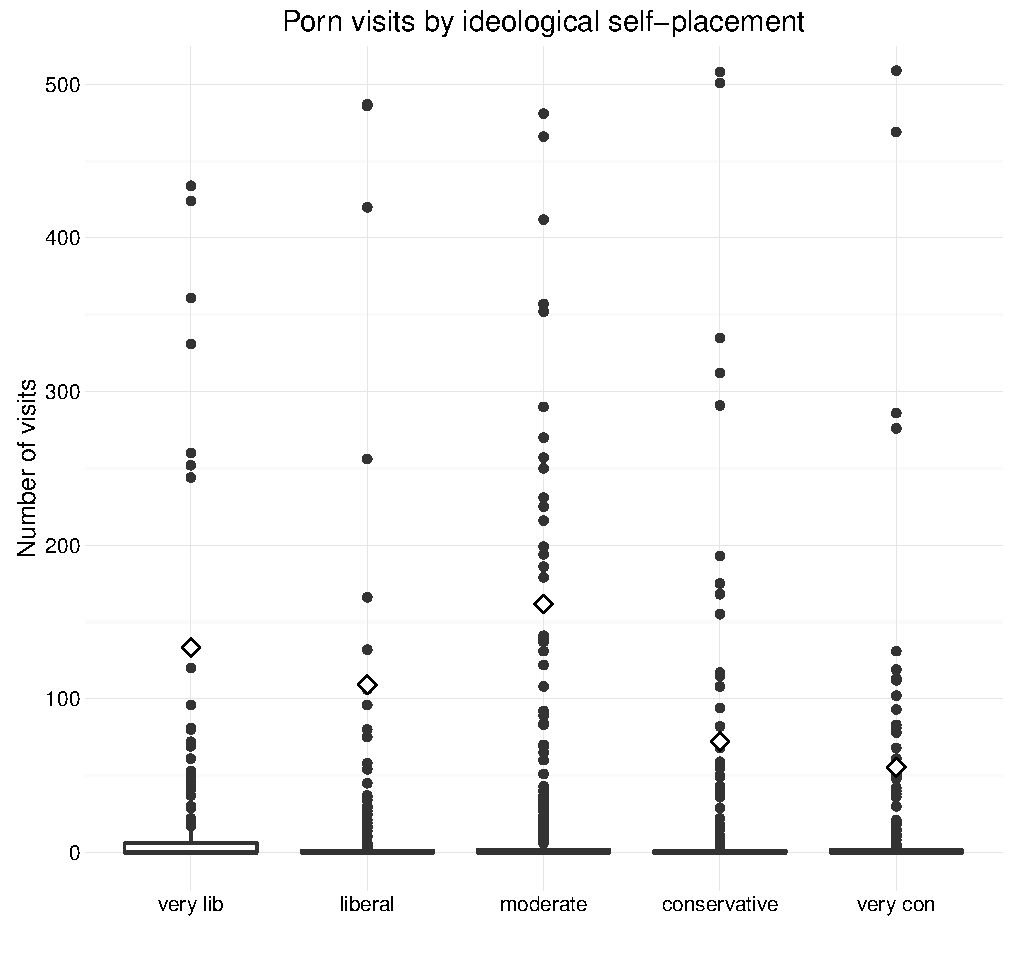
\includegraphics[scale=.75]{../figs/ideo_boxplot_shalla.pdf}
\label{fig:summary}
\end{figure}

\section*{Discussion}

\clearpage
\bibliographystyle{apsr}
\bibliography{porn_bib}
\clearpage
\appendix
\renewcommand{\thesection}{SI \arabic{section}}
\renewcommand\thetable{\thesection.\arabic{table}}  
\renewcommand\thefigure{\thesection.\arabic{figure}}
\counterwithin{figure}{section}
\counterwithin{table}{section}

\begin{center}
\Large{Supporting Information}
\end{center}


\section{Comparing comScore Sample to Population Benchmarks}
\label{si1_comscore}
% latex table generated in R 3.3.1 by xtable 1.8-2 package
% Thu Oct 27 18:50:52 2016
\begin{table}[!htb]
\centering
\caption{comScore Demographics} 
\label{tab:cs_dem}
\begingroup\tiny
\begin{tabular}{rrrrrrrrrrr}
  \hline
 & 2002 & 2004 & 2006 & 2007 & 2008 & 2009 & 2010 & 2011 & 2012 & 2013 \\ 
  \hline
Less than HS & 1.44 & 1.98 & 0.18 & 0.03 & 0.01 & 0.01 & 0.00 & 0.00 & 0.00 & 0.00 \\ 
  HS Diploma or Equivalent & 13.12 & 15.62 & 6.92 & 7.77 & 0.76 & 0.18 & 0.00 & 0.00 & 0.00 & 2.88 \\ 
  Some college but no degree & 24.97 & 19.49 & 7.16 & 8.37 & 0.75 & 0.21 & 0.00 & 0.00 & 0.00 & 18.81 \\ 
  Associate & 7.07 & 7.47 & 0.72 & 0.13 & 0.06 & 0.03 & 0.00 & 0.00 & 0.00 & 15.38 \\ 
  BS & 13.32 & 11.18 & 3.74 & 6.54 & 0.59 & 0.14 & 0.00 & 0.00 & 0.00 & 10.59 \\ 
  Grad. Degree or Above & 8.16 & 6.09 & 3.65 & 4.28 & 0.42 & 0.08 & 0.00 & 0.00 & 0.00 & 0.59 \\ 
  less Than 15k & 6.38 & 7.17 & 10.09 & 12.84 & 13.75 & 15.76 & 13.44 & 13.18 & 16.97 & 11.79 \\ 
  15k--25k & 11.72 & 10.34 & 7.02 & 8.26 & 7.83 & 10.02 & 9.18 & 7.31 & 11.71 & 9.65 \\ 
  25k--35k & 15.56 & 16.15 & 11.48 & 10.21 & 9.74 & 10.44 & 10.24 & 9.96 & 12.37 & 10.58 \\ 
  35k--50k & 20.12 & 21.24 & 20.68 & 14.75 & 11.24 & 11.31 & 13.75 & 15.18 & 14.16 & 15.82 \\ 
  50k--75k & 24.38 & 24.08 & 25.34 & 22.34 & 22.74 & 21.50 & 25.08 & 26.23 & 21.10 & 21.38 \\ 
  75k--100k & 10.87 & 10.94 & 11.78 & 13.95 & 15.26 & 14.63 & 14.12 & 13.97 & 11.60 & 13.04 \\ 
  100k+ & 10.98 & 10.08 & 13.61 & 17.66 & 19.43 & 16.33 & 14.19 & 14.17 & 12.10 & 17.74 \\ 
  18--20 & 3.22 & 1.19 & 0.33 & 0.28 & 0.49 & 0.40 & 0.66 & 4.15 & 4.17 & 4.90 \\ 
  21--24 & 5.78 & 4.73 & 2.22 & 2.17 & 2.08 & 4.12 & 5.84 & 5.96 & 6.33 & 7.42 \\ 
  25--29 & 6.95 & 6.45 & 4.40 & 5.08 & 5.25 & 8.58 & 10.22 & 7.83 & 8.17 & 8.29 \\ 
  30--34 & 9.78 & 10.26 & 15.13 & 9.94 & 7.48 & 8.44 & 9.05 & 9.20 & 9.86 & 10.03 \\ 
  35-39 & 8.99 & 10.74 & 9.25 & 11.30 & 10.41 & 11.57 & 11.85 & 9.38 & 8.63 & 8.33 \\ 
  40-44 & 11.17 & 14.57 & 19.94 & 16.12 & 14.46 & 13.17 & 12.93 & 11.59 & 11.04 & 10.47 \\ 
  45-49 & 17.36 & 15.32 & 11.90 & 14.81 & 17.62 & 15.26 & 15.13 & 12.78 & 12.35 & 11.91 \\ 
  50-54 & 15.16 & 13.20 & 11.92 & 13.33 & 14.81 & 12.77 & 11.63 & 12.07 & 11.68 & 11.72 \\ 
  55-59 & 7.45 & 8.35 & 8.38 & 9.55 & 9.97 & 8.95 & 7.75 & 8.97 & 9.18 & 8.99 \\ 
  60-64 & 6.25 & 5.98 & 6.44 & 6.98 & 6.97 & 6.80 & 6.00 & 6.82 & 6.69 & 6.60 \\ 
  65+ & 7.89 & 9.19 & 10.02 & 10.43 & 10.46 & 9.94 & 8.93 & 11.26 & 11.90 & 11.33 \\ 
  White & 82.15 & 79.88 & 93.86 & 94.08 & 86.24 & 80.11 & 79.26 & 58.73 & 54.39 & 45.44 \\ 
  Black & 6.82 & 9.01 & 4.41 & 4.62 & 8.90 & 10.99 & 12.40 & 23.12 & 20.31 & 23.52 \\ 
  Asian & 4.12 & 3.32 & 1.14 & 1.13 & 1.28 & 1.33 & 1.43 & 3.89 & 8.26 & 6.35 \\ 
  Other & 6.91 & 7.79 & 0.54 & 0.17 & 3.58 & 7.57 & 6.91 & 14.26 & 17.04 & 24.69 \\ 
  Hispanic & 8.84 & 14.33 & 21.19 & 23.12 & 27.14 & 9.76 & 7.56 & 10.81 & 12.58 & 15.89 \\ 
  Non-Hispanic & 91.16 & 85.67 & 78.81 & 76.88 & 72.86 & 90.24 & 92.44 & 89.19 & 87.42 & 84.11 \\ 
  Northeast & 18.71 & 18.69 & 17.69 & 19.21 & 19.64 & 18.25 & 17.65 & 17.75 & 18.12 & 19.44 \\ 
  North Central & 23.48 & 22.16 & 22.65 & 22.14 & 21.77 & 19.85 & 19.38 & 19.52 & 20.03 & 19.14 \\ 
  South & 37.07 & 37.89 & 39.34 & 38.48 & 38.68 & 39.06 & 39.92 & 40.09 & 39.35 & 39.07 \\ 
  West & 20.74 & 21.27 & 19.57 & 19.57 & 19.23 & 20.08 & 20.01 & 22.01 & 22.44 & 22.32 \\ 
  Broadband & 40.42 & 28.38 & 77.11 & 86.86 & 93.93 & 97.07 & 98.52 & 96.49 & 96.76 & 99.06 \\ 
  Not Broadband & 59.58 & 71.62 & 22.89 & 13.14 & 6.07 & 2.93 & 1.48 & 3.51 & 3.24 & 0.94 \\ 
   \hline
\end{tabular}
\endgroup
\end{table}


\clearpage
\section{Comparing YouGov Sample to Population Benchmarks}
\label{si2_yougov}

% latex table generated in R 3.3.0 by xtable 1.8-2 package
% Thu Jun  2 17:50:30 2016
\begin{table}[ht]
\centering
\begin{tabular}{rrrr}
  \hline
 & Unweighted & Weighted & Population \\ 
  \hline
18-24 & 0.03 & 0.13 & 0.13 \\ 
  25-44 & 0.30 & 0.34 & 0.34 \\ 
  45-64 & 0.59 & 0.34 & 0.34 \\ 
  65+ & 0.07 & 0.19 & 0.19 \\ 
  female & 0.56 & 0.51 & 0.51 \\ 
  male & 0.44 & 0.49 & 0.49 \\ 
  asian & 0.04 & 0.05 & 0.05 \\ 
  black & 0.09 & 0.12 & 0.12 \\ 
  hispanic & 0.05 & 0.14 & 0.14 \\ 
  other & 0.07 & 0.05 & 0.05 \\ 
  white & 0.76 & 0.64 & 0.64 \\ 
  ind & 0.28 & 0.39 & 0.39 \\ 
  dem & 0.37 & 0.32 & 0.32 \\ 
  oth/dk & 0.12 & 0.06 & 0.06 \\ 
  rep & 0.23 & 0.23 & 0.23 \\ 
  midwest & 0.24 & 0.22 & 0.22 \\ 
  northeast & 0.18 & 0.18 & 0.18 \\ 
  south & 0.34 & 0.37 & 0.37 \\ 
  west & 0.24 & 0.23 & 0.23 \\ 
  $<$ \$20,000 & 0.16 & 0.14 & 0.13 \\ 
  $>$= \$120,000 & 0.09 & 0.10 & 0.11 \\ 
  \$100,000-119,999 & 0.06 & 0.06 & 0.14 \\ 
  \$20,000-39,999 & 0.25 & 0.25 & 0.17 \\ 
  \$40,000-59,999 & 0.22 & 0.23 & 0.08 \\ 
  \$60,000-79,999 & 0.14 & 0.15 & 0.20 \\ 
  \$80,000-99,999 & 0.08 & 0.06 & 0.17 \\ 
   \hline
\end{tabular}
\end{table}


\end{document}
